\documentclass[tikz,border=12pt]{standalone}
\usepackage[scaled=0.95]{helvet}
\renewcommand{\familydefault}{\sfdefault}
\usepackage[T1]{fontenc}
\usetikzlibrary{arrows.meta,positioning,calc}

\definecolor{ink}{HTML}{16324F}
\definecolor{band}{HTML}{F7F9FB}
\definecolor{bandB}{HTML}{B9C6D2}
\definecolor{box}{HTML}{DCEAF7}
\definecolor{boxB}{HTML}{2F6DA8}
\definecolor{agent}{HTML}{E9E1F5}
\definecolor{agentB}{HTML}{6B46A8}
\definecolor{ok}{HTML}{1F8A7A}

\tikzset{
  b/.style={rounded corners=3pt,fill=box,draw=boxB,line width=0.8pt,minimum height=1.15cm,
    align=center,font=\footnotesize,text=ink},
  layer/.style={rounded corners=5pt,fill=band,draw=bandB,line width=0.8pt,minimum width=20.4cm,anchor=west},
  lt/.style={anchor=west,font=\footnotesize\bfseries,text=ink,align=left,text width=2.5cm},
  flow/.style={-{Stealth[length=3mm]},line width=1.2pt,draw=ink},
}
\newcommand{\cname}[2]{\textbf{#1}\\[-1pt]{\scriptsize #2}}

\begin{document}
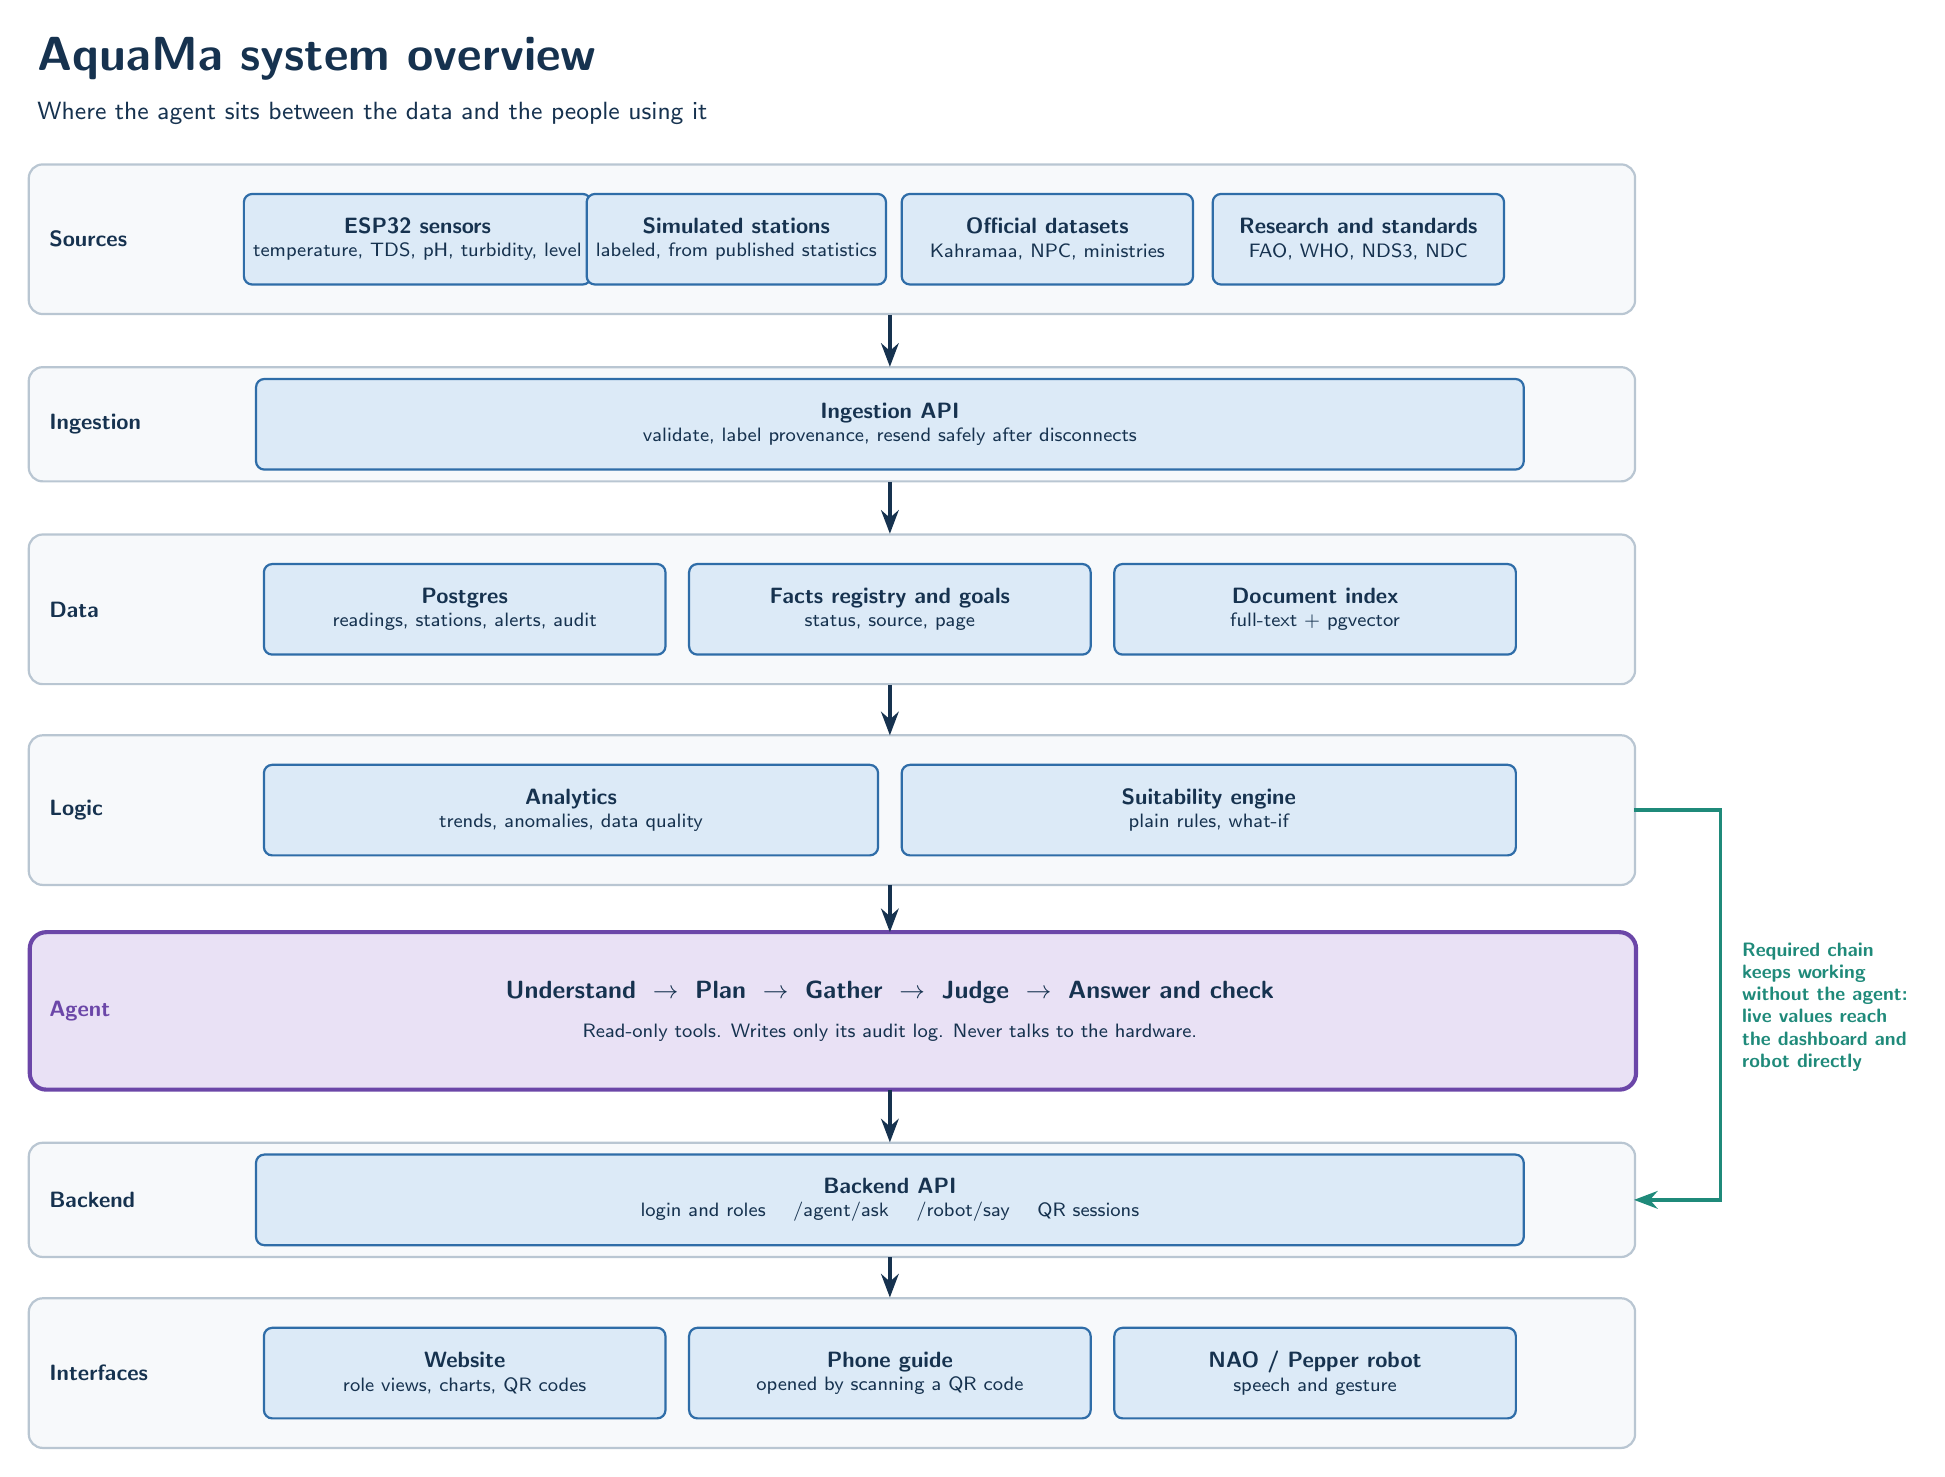
\begin{tikzpicture}

\node[anchor=west,font=\LARGE\bfseries,text=ink] at (0,17.6) {AquaMa system overview};
\node[anchor=west,font=\small,text=ink] at (0,16.9) {Where the agent sits between the data and the people using it};

% layers
\foreach \y/\h/\t in {15.3/1.9/Sources,12.95/1.45/Ingestion,10.6/1.9/Data,8.05/1.9/Logic,3.1/1.45/Backend,0.9/1.9/Interfaces}{
  \node[layer,minimum height=\h cm] at (0,\y) {};
  \node[lt] at (0.15,\y) {\t};
}

% sources
\node[b,minimum width=3.9cm] (s1) at (4.95,15.3)  {\cname{ESP32 sensors}{temperature, TDS, pH, turbidity, level}};
\node[b,minimum width=3.7cm] (s2) at (9.0,15.3)  {\cname{Simulated stations}{labeled, from published statistics}};
\node[b,minimum width=3.7cm] (s3) at (12.95,15.3) {\cname{Official datasets}{Kahramaa, NPC, ministries}};
\node[b,minimum width=3.7cm] (s4) at (16.9,15.3){\cname{Research and standards}{FAO, WHO, NDS3, NDC}};

% ingestion
\node[b,minimum width=16.1cm] (ing) at (10.95,12.95) {\cname{Ingestion API}{validate, label provenance, resend safely after disconnects}};

% data
\node[b,minimum width=5.1cm] (d1) at (5.55,10.6)  {\cname{Postgres}{readings, stations, alerts, audit}};
\node[b,minimum width=5.1cm] (d2) at (10.95,10.6) {\cname{Facts registry and goals}{status, source, page}};
\node[b,minimum width=5.1cm] (d3) at (16.35,10.6) {\cname{Document index}{full-text + pgvector}};

% logic
\node[b,minimum width=7.8cm] (l1) at (6.9,8.05)  {\cname{Analytics}{trends, anomalies, data quality}};
\node[b,minimum width=7.8cm] (l2) at (15.0,8.05) {\cname{Suitability engine}{plain rules, what-if}};

% agent
\node[rounded corners=6pt,fill=agent,draw=agentB,line width=1.5pt,minimum width=20.4cm,minimum height=2.0cm,anchor=west] (ag) at (0,5.5) {};
\node[lt,text=agentB] at (0.15,5.5) {Agent};
\node[align=center,font=\small,text=ink] at (10.95,5.5) {\textbf{Understand \;$\rightarrow$\; Plan \;$\rightarrow$\; Gather \;$\rightarrow$\; Judge \;$\rightarrow$\; Answer and check}\\[3pt]{\scriptsize Read-only tools. Writes only its audit log. Never talks to the hardware.}};

% backend
\node[b,minimum width=16.1cm] (api) at (10.95,3.1) {\cname{Backend API}{login and roles \quad /agent/ask \quad /robot/say \quad QR sessions}};

% interfaces
\node[b,minimum width=5.1cm] (i1) at (5.55,0.9)  {\cname{Website}{role views, charts, QR codes}};
\node[b,minimum width=5.1cm] (i2) at (10.95,0.9) {\cname{Phone guide}{opened by scanning a QR code}};
\node[b,minimum width=5.1cm] (i3) at (16.35,0.9) {\cname{NAO / Pepper robot}{speech and gesture}};

% flows
\foreach \a in {14.34}{ \draw[flow] (10.95,14.34)--(10.95,13.68); }
\draw[flow] (10.95,12.22)--(10.95,11.56);
\draw[flow] (10.95,9.64)--(10.95,9.0);
\draw[flow] (10.95,7.1)--(10.95,6.5);
\draw[flow] (10.95,4.5)--(10.95,3.83);
\draw[flow] (10.95,2.37)--(10.95,1.86);

% required path
\draw[-{Stealth[length=3mm]},line width=1.3pt,draw=ok] (20.4,8.05)--(21.5,8.05)--(21.5,3.1)--(20.4,3.1);
\node[font=\scriptsize\bfseries,text=ok,align=left,anchor=west] at (21.65,5.55) {Required chain\\keeps working\\without the agent:\\live values reach\\the dashboard and\\robot directly};

\end{tikzpicture}
\end{document}
